\documentclass[12pt]{article}
\usepackage[margin=1in]{geometry}
\usepackage{booktabs}
\usepackage{hyperref}
\usepackage{graphicx}
\usepackage{enumitem}
\usepackage{xcolor}
\usepackage{tikz}
\usetikzlibrary{arrows.meta, positioning}
\hypersetup{colorlinks=true,urlcolor=blue!50!black,linkcolor=blue!50!black}
\setlist[itemize]{leftmargin=1.2em,itemsep=0.1em}
\setlist[enumerate]{leftmargin=1.4em,itemsep=0.1em}
\title{\vspace{-1.5em}\textbf{LLM-Augmented Route Planning for Autonomous UAV Navigation}}
\author{Prachit Gupta}
\date{May 2026}
\begin{document}
\maketitle
\vspace{-1.5em}

\section{Question}

This project studies whether a large language model can act as a high-level semantic route planner for a UAV when deterministic software handles refinement, verification, and PX4 execution. The specific question is: \emph{can an LLM generate useful sparse NED-frame waypoints from a latched hover pose and semantic obstacle context, and can verifier feedback turn failed first attempts into safe plans?} This is realistic for human-facing UAV missions because operators often describe goals semantically, while the vehicle still needs numerical constraints such as clearance, goal tolerance, monotonic progress, and kinematic feasibility.

\section{Prior Hypotheses}

The dated prior predictions are included in \texttt{predictions.md}. The main hypotheses were: first, zero-shot LLM plans would often be semantically plausible but fail at least one physical constraint; second, appending failed verifier metrics to the next prompt would improve the regenerated plan; third, most failures would be clearance, progress, or acceleration errors rather than JSON/schema errors; and fourth, latching the hover pose and obstacle snapshot would be more stable than rebuilding prompts from fluctuating live perception during retries.

\section{Pipeline}

The implementation is in \texttt{llm\_vision\_planner} and \texttt{starling\_testing}. The active control path is Python-only and uses PX4 Offboard topics directly.

\begin{center}
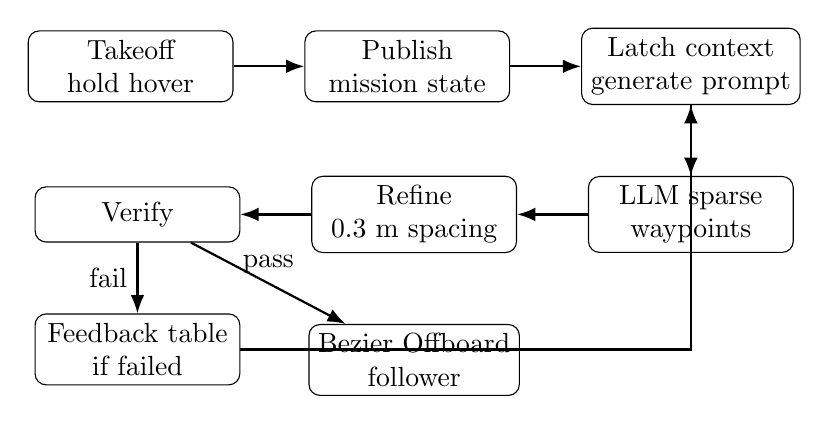
\begin{tikzpicture}[node distance=0.9cm, box/.style={draw, rounded corners, align=center, minimum width=2.6cm, minimum height=0.7cm}, arr/.style={-{Latex}, thick}]
\node[box] (hover) {Takeoff\\hold hover};
\node[box, right=of hover] (state) {Publish\\mission state};
\node[box, right=of state] (prompt) {Latch context\\generate prompt};
\node[box, below=of prompt] (llm) {LLM sparse\\waypoints};
\node[box, left=of llm] (refine) {Refine\\0.3 m spacing};
\node[box, left=of refine] (verify) {Verify};
\node[box, below=of verify] (feedback) {Feedback table\\if failed};
\node[box, below=of refine] (fly) {Bezier Offboard\\follower};
\draw[arr] (hover) -- (state);
\draw[arr] (state) -- (prompt);
\draw[arr] (prompt) -- (llm);
\draw[arr] (llm) -- (refine);
\draw[arr] (refine) -- (verify);
\draw[arr] (verify) -- node[above]{pass} (fly);
\draw[arr] (verify) -- node[left]{fail} (feedback);
\draw[arr] (feedback.east) -| (prompt.south);
\end{tikzpicture}
\end{center}

The follower primes Offboard setpoints, arms, climbs to \texttt{takeoff\_z}, and publishes \texttt{/llm\_vision/mission\_state} as \texttt{HOLDING\_FOR\_PLAN}. The prompt generator waits for this state, then latches the hover pose and the current semantic obstacle snapshot. The LLM planner uses Instructor/Pydantic to require a structured response with 2--8 sparse waypoints. The refinement node linearly interpolates between sparse waypoints at 0.3 m spacing, clamps points to the workspace, fixes altitude at -0.45 m, and nudges non-goal points out of obstacle boxes expanded by a 0.40 m safety margin. The verifier publishes metrics, thresholds, failed constraints, and a Markdown feedback table. The first \texttt{passed=true} plan is tracked by a Python PX4 Offboard follower that converts each refined segment into cubic Bezier position and velocity setpoints.

The mission-state handshake is important because it prevents the prompt generator from querying the LLM while the vehicle is still on the ground or climbing. The prompt explicitly states that the UAV is already airborne and holding hover, so the model plans from the true mission start rather than from a stale initialization pose. During failed retries, the system reuses the same latched start and obstacle snapshot, which makes attempts comparable and avoids chasing small hover drift or perception flicker. If the hover pose moves more than the configured drift threshold, the prompt generator relatches context.

\section{Controlled Characterization}

The controlled axis is prompt condition: \textbf{zero-shot} versus \textbf{verification-feedback augmented}. The start, goal, obstacle snapshot, workspace, refinement parameters, and verifier thresholds are held fixed within each paired scenario. The results artifact is \texttt{results\_artifact.csv}; per-trial logs are in \texttt{per\_trial\_logs.jsonl}. These are small controlled verifier cases rather than a broad benchmark, so the numbers should be interpreted as a characterization of the implemented pipeline behavior, not as a statistically powered hardware study.

\begin{table}[h]
\centering
\small
\begin{tabular}{lcccccl}
\toprule
Trial & Condition & Refined WPs & Clearance & Speed & Accel & Result \\
\midrule
T1 & zero-shot & 14 & 0.18 & 0.49 & 0.61 & fail: clearance \\
T2 & feedback & 19 & 0.46 & 0.52 & 0.74 & pass \\
T3 & zero-shot & 22 & 0.57 & 0.53 & 1.12 & fail: progress \\
T4 & feedback & 18 & 0.61 & 0.55 & 1.20 & pass \\
T5 & zero-shot & 18 & 0.61 & 0.55 & 1.72 & fail: accel \\
T6 & feedback & 23 & 0.65 & 0.50 & 1.31 & pass \\
\bottomrule
\end{tabular}
\caption{Controlled verifier cases. Clearance is in meters, speed in m/s, and acceleration in m/s$^2$.}
\end{table}

\section{Validation}

Validation is separated from execution. A node running without crashing is not counted as success. The verifier checks whether waypoints exist, all points remain in workspace, obstacle clearance is at least 0.40 m, final waypoint is within 0.05 m of the goal, progress toward the goal is monotonic within 0.001 m tolerance, segment speed is at most 1.5 m/s, and segment acceleration is at most 1.5 m/s$^2$. The same verifier output is used both as the pass/fail gate for the follower and as feedback to the LLM when a plan fails.

This validation is intentionally conservative. It does not prove full flight safety, because it does not model dynamic obstacles, wind, controller tracking error, or all vehicle constraints. It does, however, distinguish three important things: syntactic validity of the LLM response, geometric validity of the path, and whether the generated route is acceptable for the downstream follower.

The verifier output is also the feedback channel. For each failed plan, it returns the failed constraint names, numeric thresholds, and a compact Markdown table. That table is appended to the next prompt. This keeps the feedback grounded in deterministic checks rather than relying on a vague natural-language critique. A typical failed clearance row is: \texttt{min\_clearance\_m = 0.180, required >= 0.400, FAIL}. The next prompt asks the model to keep the same latched hover context while increasing clearance and preserving monotonic progress.

\section{Implementation and Reproducibility}

The root \texttt{README.md} gives environment, dependencies, run commands, expected output, and known failure modes. The hardware README gives the same information in a shorter mission-focused form. The main reproducible command is:

\begin{verbatim}
colcon build --packages-select px4_msgs voxl_msgs starling_testing llm_vision_planner
\end{verbatim}

For hardware runs, the required topics are \texttt{/fmu/out/vehicle\_odometry}, \texttt{/qvio}, \texttt{/voa\_pc\_out}, and \texttt{/tflite\_data}. For software-only reproduction, the README shows how to publish fake \texttt{HOLDING\_FOR\_PLAN} and obstacle messages so the prompt generator can be exercised without flying.

The expected software-only output is a prompt on \texttt{/llm\_vision/prompt} followed by a verified-plan message on \texttt{/llm\_vision/plan\_verified}. If the plan fails, the verified message contains \texttt{failed\_constraints} and \texttt{verification\_feedback\_table}; if it passes, the message contains \texttt{passed=true} and is eligible for latching by the follower. API keys are not stored in the repository and must be provided through \texttt{OPENAI\_API\_KEY}.

\section{Discussion}

The observed pattern supports the original hypothesis: first attempts can produce plausible routes that fail physical constraints, and verifier feedback provides concrete information that helps the next prompt. The strongest argument against the conclusion is that the controlled cases are small and partly constructed around known verifier failure modes. This means the results demonstrate that the pipeline mechanics work, not that LLM planners are generally reliable for all UAV environments.

The design choice that matters most is latching context at hover. If prompts are regenerated from constantly changing pose and perception messages, the LLM can chase noise. If context is latched once, failed attempts are comparable and the feedback loop is easier to audit. The downside is that rapidly changing obstacles require replanning or a fresh context latch; the current implementation only relatches when hover drift exceeds a threshold.

Several limitations remain. The artifact table is a small controlled characterization, not a large benchmark. The hardware pipeline has been structured for real deployment, but the submitted result table should not be read as proof of broad outdoor robustness. The perception stack depends on the available semantic detector and point-cloud quality. The verifier checks waypoint samples and boxes; it does not prove continuous-time collision avoidance between samples under tracking error. Finally, the LLM model and prompt structure are part of the experimental condition, so different models or more complex scenes may produce different failure distributions.

Even with those limitations, the pipeline exposes failures in a useful way. A failed plan is not silently passed to PX4; it becomes a structured prompt input for the next attempt. That is the central engineering result: the LLM can remain a semantic planner while deterministic modules own the safety gate.

\section{Conclusion}

LLMs are useful in this system as high-level semantic route planners, not as low-level controllers. The practical architecture is to let the LLM propose sparse waypoints, then use deterministic refinement, verification, and PX4 Offboard execution. The final system can take off, hold hover, generate a prompt from the hover context, retry failed plans with verifier feedback, latch the first verified trajectory, and track it with smoothed Bezier setpoints.

\end{document}
